% ---------------------------------------------------------------------------
% Author guideline and sample document for EG publication using LaTeX2e input
% D.Fellner, v1.13, Jul 31, 2008

\documentclass{egpubl}
\usepackage{eurovis2019}

% --- for  Annual CONFERENCE
% \ConferenceSubmission   % uncomment for Conference submission
% \ConferencePaper        % uncomment for (final) Conference Paper
% \STAR                   % uncomment for STAR contribution
% \Tutorial               % uncomment for Tutorial contribution
% \ShortPresentation      % uncomment for (final) Short Conference Presentation
% \Areas                  % uncomment for Areas contribution
% \MedicalPrize           % uncomment for Medical Prize contribution
% \Education              % uncomment for Education contribution
% \Poster                 % uncomment for Poster contribution
% \DC                     % uncomment for Doctoral Consortium
%
% --- for  CGF Journal
% \JournalSubmission    % uncomment for submission to Computer Graphics Forum
% \JournalPaper         % uncomment for final version of Journal Paper
%
% --- for  CGF Journal: special issue
% \SpecialIssueSubmission    % uncomment for submission to , special issue
% \SpecialIssuePaper         % uncomment for final version of Computer Graphics Forum, special issue
%                          % EuroVis, SGP, Rendering, PG
% --- for  EG Workshop Proceedings
% \WsSubmission      % uncomment for submission to EG Workshop
% \WsPaper           % uncomment for final version of EG Workshop contribution
% \WsSubmissionJoint % for joint events, for example ICAT-EGVE
% \WsPaperJoint      % for joint events, for example ICAT-EGVE
% \Expressive        % for SBIM, CAe, NPAR
% \DigitalHeritagePaper
% \PaperL2P          % for events EG only asks for License to Publish

% --- for EuroVis 
% for full papers use \SpecialIssuePaper
% \STAREurovis   % for EuroVis additional material 
\EuroVisPoster % for EuroVis additional material 
% \EuroVisShort  % for EuroVis additional material

 \electronicVersion % can be used both for the printed and electronic version

% !! *please* don't change anything above
% !! unless you REALLY know what you are doing
% ------------------------------------------------------------------------

% for including postscript figures
% mind: package option 'draft' will replace PS figure by a filename within a frame
\ifpdf \usepackage[pdftex]{graphicx} \pdfcompresslevel=9
\else \usepackage[dvips]{graphicx} \fi

\PrintedOrElectronic

% prepare for electronic version of your document
\usepackage{t1enc,dfadobe}

\usepackage{egweblnk}
\usepackage{cite}

% For backwards compatibility to old LaTeX type font selection.
% Uncomment if your document adheres to LaTeX2e recommendations.
% \let\rm=\rmfamily    \let\sf=\sffamily    \let\tt=\ttfamily
% \let\it=\itshape     \let\sl=\slshape     \let\sc=\scshape
% \let\bf=\bfseries

% end of prologue
% ---------------------------------------------------------------------
% EG author guidelines plus sample file for EG publication using LaTeX2e input
% D.Fellner, v2.02, Jan 25, 2017


\title[Improving the Scalability of Interactive Visualization Systems for Exploring Threaded Conversations]%
      {Improving the Scalability of Interactive Visualization Systems for Exploring Threaded Conversations}

% for anonymous conference submission please enter your SUBMISSION ID
% instead of the author's name (and leave the affiliation blank) !!
% for final version: please provide your *own* ORCID in the brackets following \orcid; see https://orcid.org/ for more details.
\author[A. McNutt \& G. Kindlmann]
{\parbox{\textwidth}{\centering A. McNutt, IEEE student member, \& G. Kindlmann
%        S. Spencer$^2$\thanks{Chairman Siggraph Publications Board}  
        }
        \\
% For Computer Graphics Forum: Please use the abbreviation of your first name.
{\parbox{\textwidth}{\centering Department of Computer Science, University of Chicago
%        $^2$ Another Department to illustrate the use in papers from authors
%             with different affiliations
       } 
}
}
% ------------------------------------------------------------------------

% if the Editors-in-Chief have given you the data, you may uncomment
% the following five lines and insert it here
%
% \volume{36}   % the volume in which the issue will be published;
% \issue{1}     % the issue number of the publication
% \pStartPage{1}      % set starting page


%-------------------------------------------------------------------------
\begin{document}

\teaser{
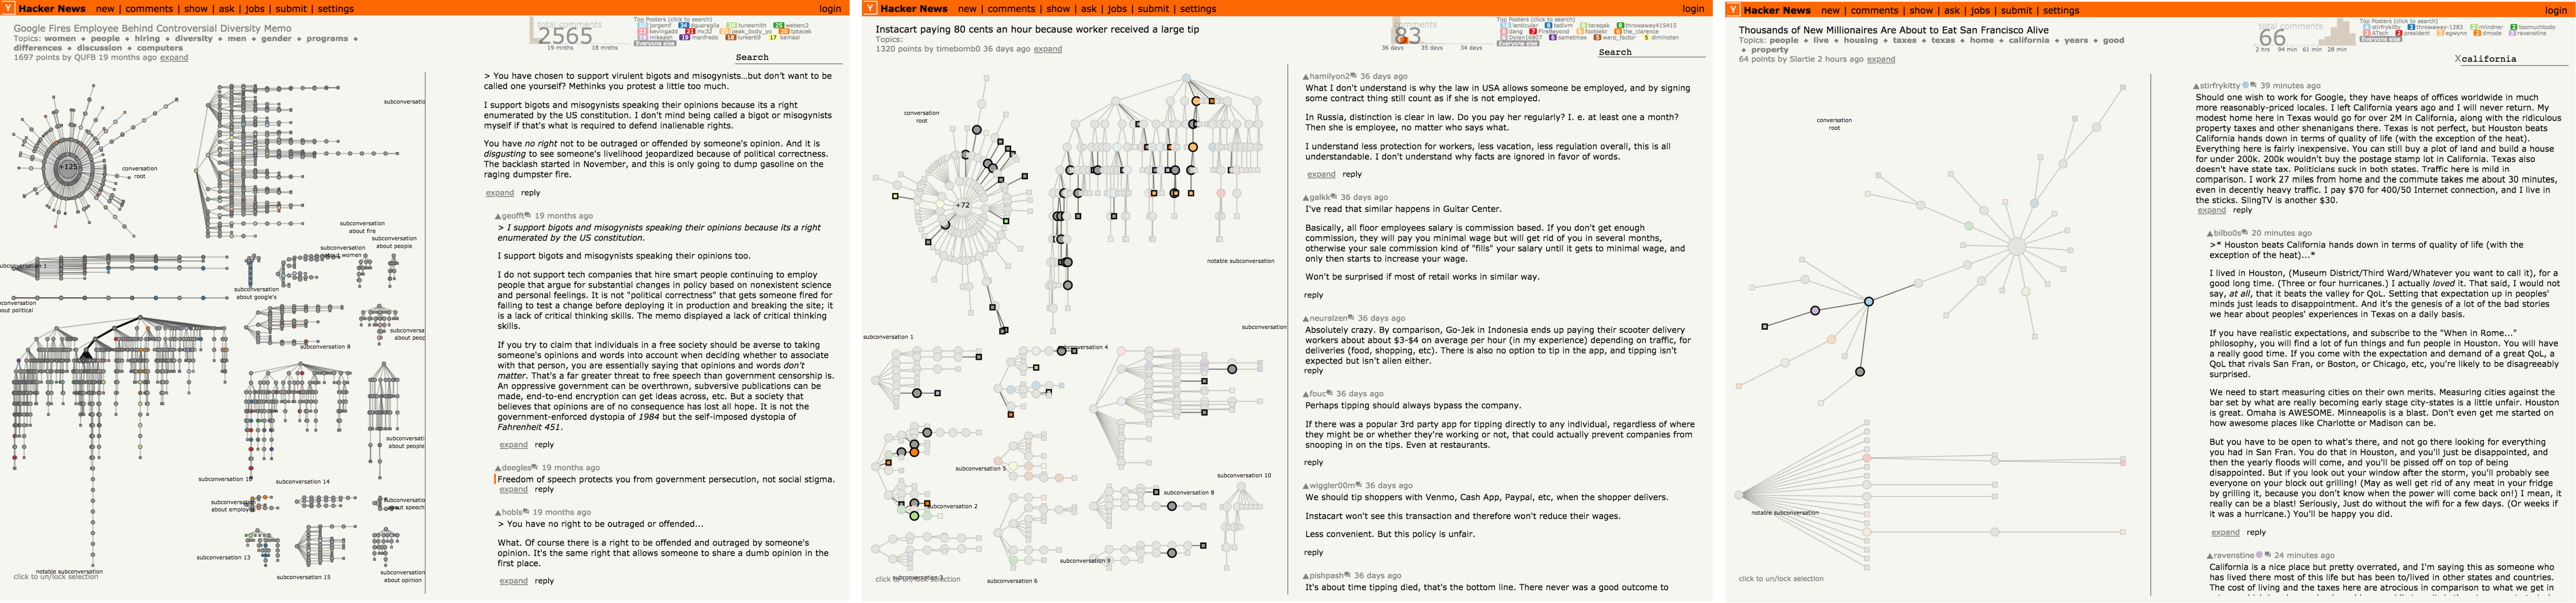
\includegraphics[width=\linewidth]{images/teaser.pdf}
\centering
\caption{
Three HackerNews conversations (left to right 715, 85, and X) rendered using our ForumExplorer application.
%
In the left image the user has moused over a particular sub-conversation; in the right they have engaged in a temporal search.
}
\label{fig:teaser}
}

\maketitle
%-------------------------------------------------------------------------
\begin{abstract}
The graphical presentation of large threaded conversations, such as those found on reddit and slashdot, presents individual comments well, but can cloak larger trends or patterns within the conversational corpus.
%
Previous works have addressed this problem through visualizations and nlp-generated summaries.
%
These works have generally been designed around an ideal size of data, which can be difficult to use for particularly large or nested conversations, and have sometimes require non-trivial offline processing time, which makes them impractical for day to day usage.
%
% In tandem these factors have likely negatively affected the adoption of this class of tool.
%
We refine these approaches by offering concrete design strategies that enable this type of representation to handle wider ranges of data, that we implement as a Chrome Extension, Forum Explorer, which facilitates practical exploration of conversations held on yCombinator's HackerNews.
%   The ABSTRACT is to be in fully-justified italicized text, 
%   between two horizontal lines,
 %  in one-column format, 
%   below the author and affiliation information. 
 %  Use the word ``Abstract'' as the title, in 9-point Times, boldface type, 
  % left-aligned to the text, initially capitalized. 
 %  The abstract is to be in 9-point, single-spaced type.
  % The abstract may be up to 3 inches (7.62 cm) long. 
  \\
%   Leave one blank line after the abstract, 
%   then add the subject categories according to the ACM Classification Index 
%-------------------------------------------------------------------------
%  ACM CCS 1998
%  (see http://www.acm.org/about/class/1998)
% \begin{classification} % according to http:http://www.acm.org/about/class/1998
% \CCScat{Computer Graphics}{I.3.3}{Picture/Image Generation}{Line and curve generation}
% \end{classification}
%-------------------------------------------------------------------------
%  ACM CCS 2012
%   (see http://www.acm.org/about/class/class/2012)
%The tool at \url{http://dl.acm.org/ccs.cfm} can be used to generate
% CCS codes.
%Example:
\begin{CCSXML}
<ccs2012>
<concept>
<concept_id>10010147.10010371.10010352.10010381</concept_id>
<concept_desc>Human-centered computing~User interface design</concept_desc>
<concept_significance>300</concept_significance>
</concept>
<concept>
<concept_id>10010583.10010588.10010559</concept_id>
<concept_desc>Human-centered computing~Visualization</concept_desc>
<concept_significance>200</concept_significance>
</concept>
<concept>
<concept_id>10010583.10010584.10010587</concept_id>
<concept_desc>Human-centered computing~Graph drawings</concept_desc>
<concept_significance>100</concept_significance>
</concept>
</ccs2012>
\end{CCSXML}

\ccsdesc[300]{Human-centered computing~User interface design}
\ccsdesc[200]{Human-centered computing~Visualization}
\ccsdesc[100]{Human-centered computing~Graph drawings}


\printccsdesc   
\end{abstract}





%-------------------------------------------------------------------------
\section{Introduction}


%%%
%%% Figure 1
%%%
\begin{figure}[htb]
\centering
% the following command controls the width of the embedded PS file
% (relative to the width of the current column)
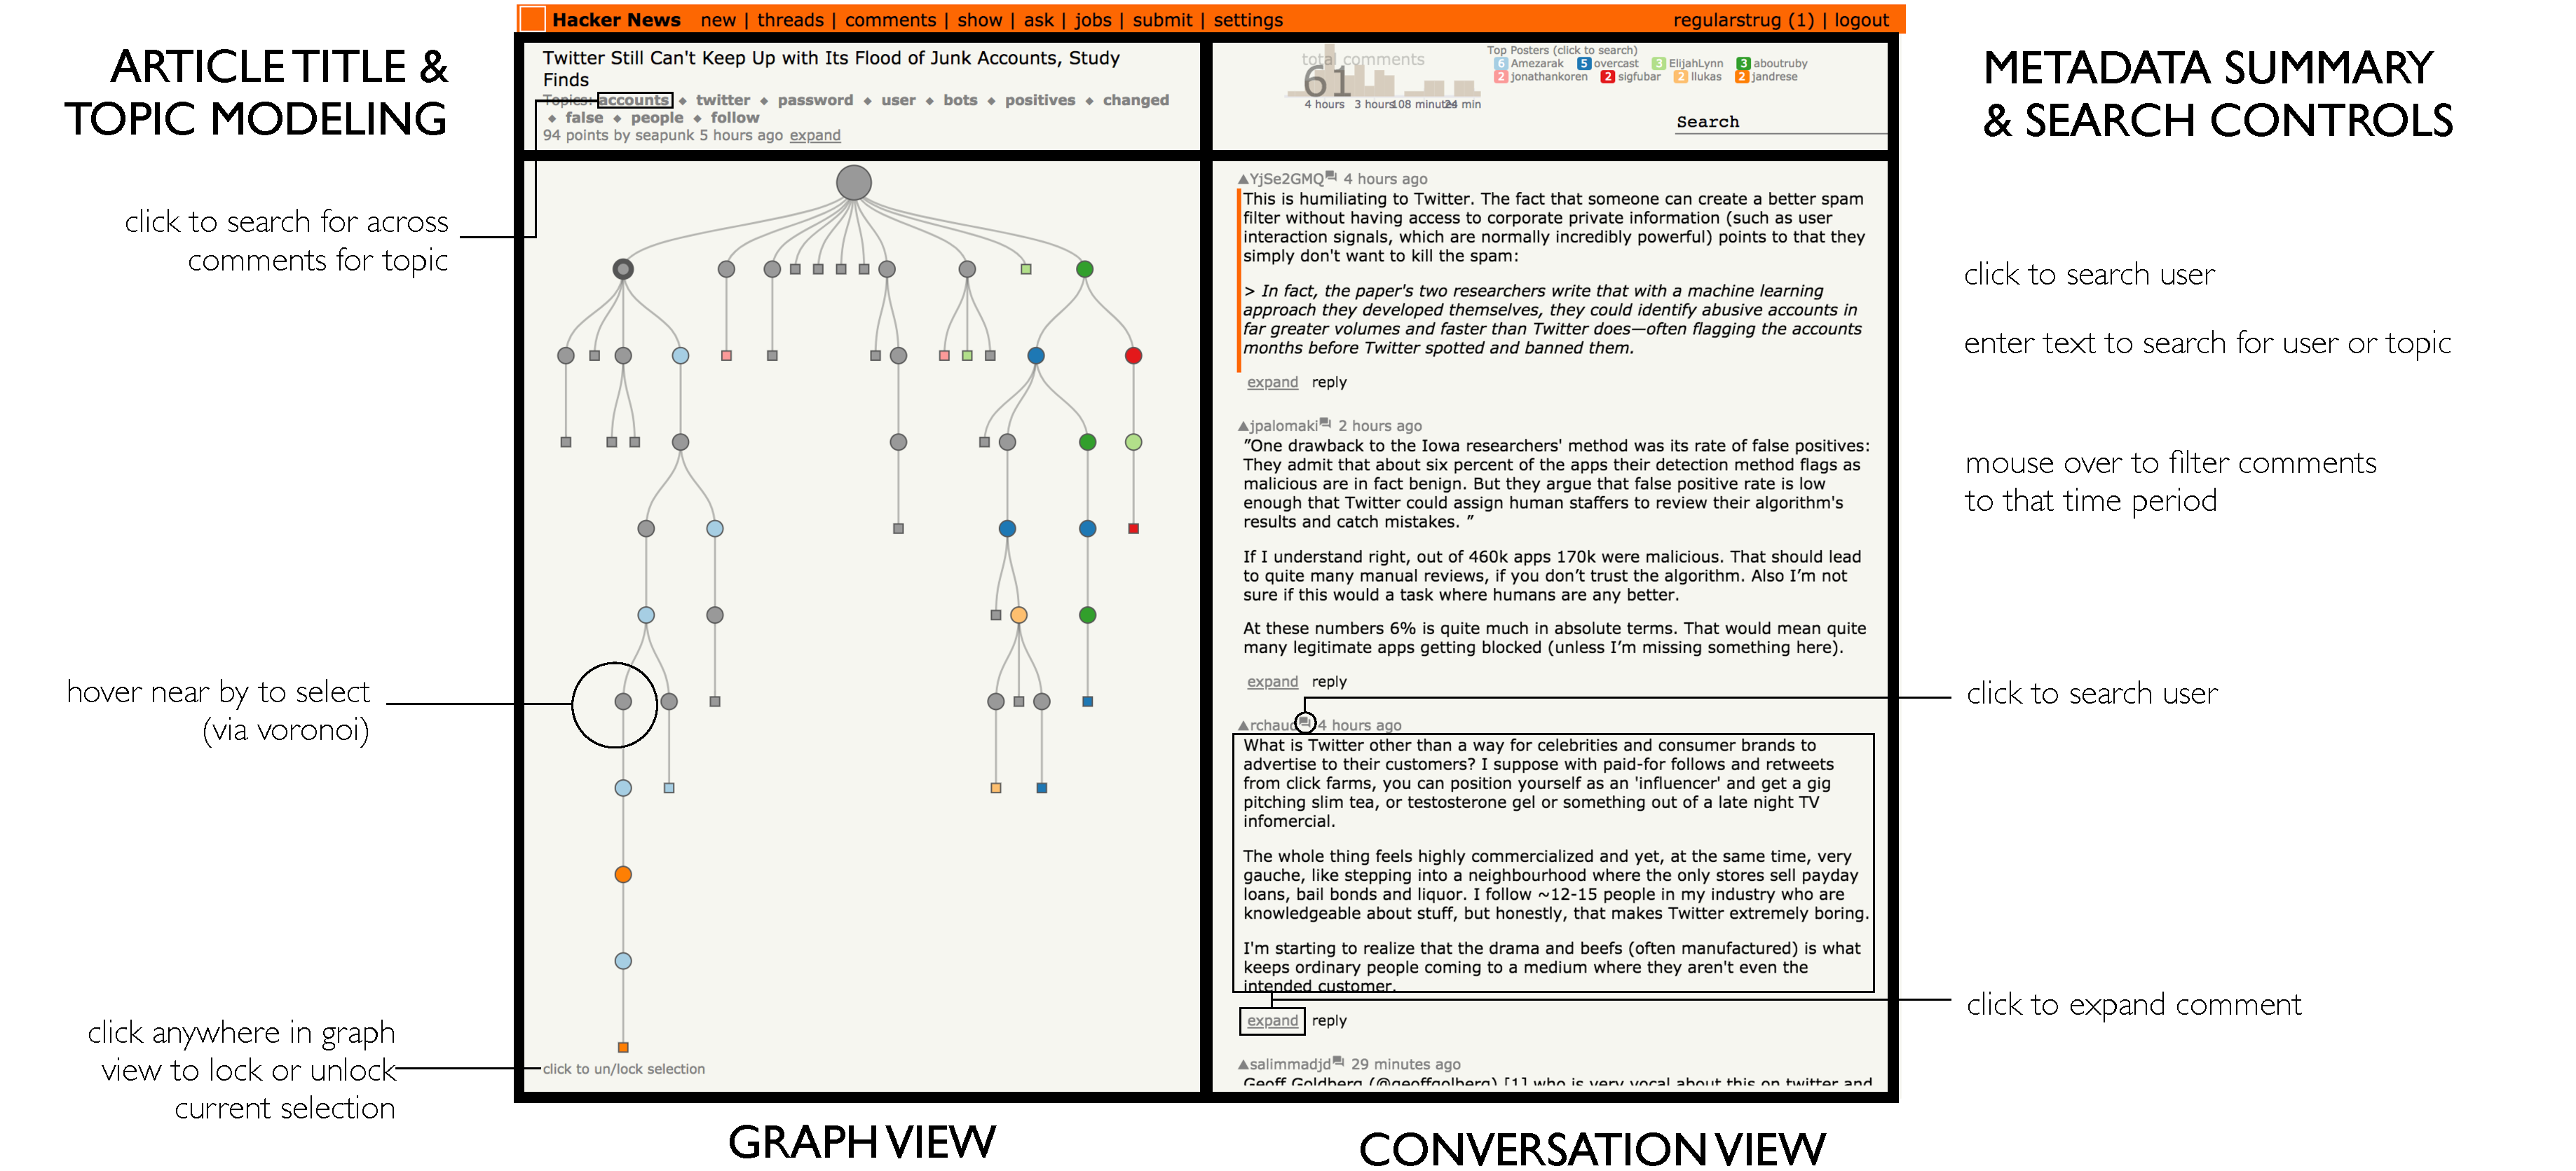
\includegraphics[width=0.9\linewidth]{images/explainer.pdf}
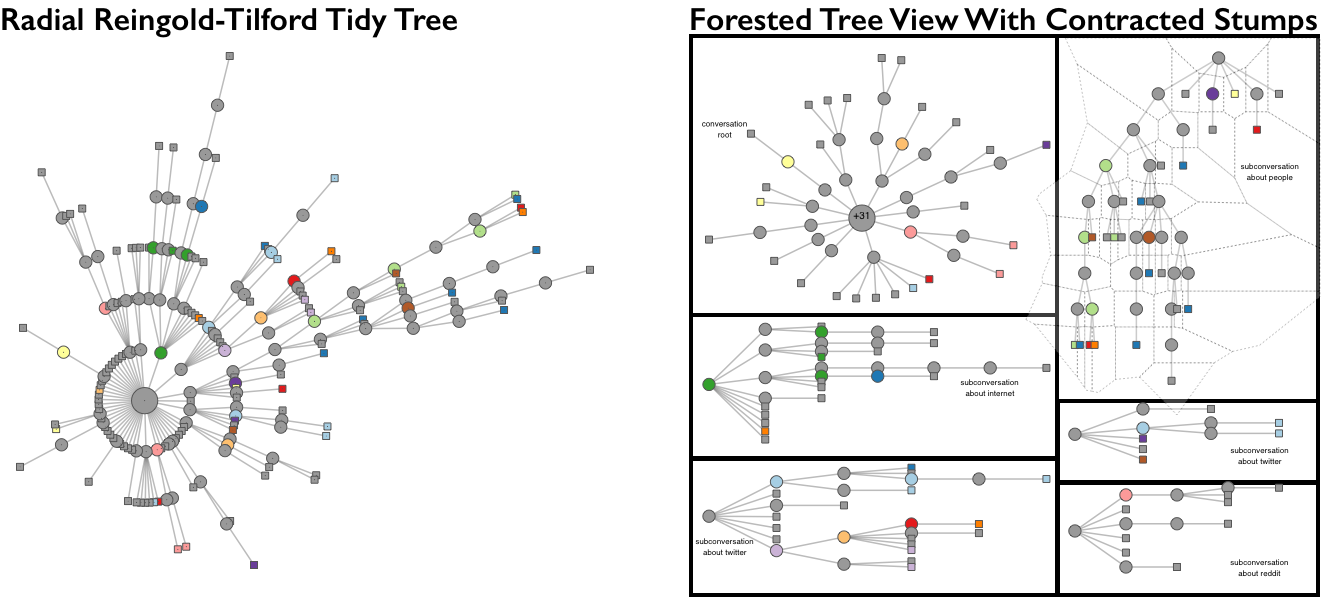
\includegraphics[width=0.9\linewidth]{images/forested-tree-view-example.png}
% replacing the above command with the one below will explicitly set
% the bounding box of the PS figure to the rectangle (xl,yl),(xh,yh).
% It will also prevent LaTeX from reading the PS file to determine
% the bounding box (i.e., it will speed up the compilation process)
% \includegraphics[width=.95\linewidth, bb=39 696 126 756]{sampleFig}
%
%  \parbox[t]{.9\columnwidth}{\relax
%          For all figures please keep in mind that you \textbf{must not}
%         use images with transparent background! 
%         }
%
\caption{
\label{fig:explainer}
Annotated view explaining the components of the UI (top) and a visual explanation of Forested Tree Layout (bottom). 
}
\end{figure}


Conversation on the internet takes many shapes and forms. 
%
Of particular interest are asynchronous threaded conversations, such as those found reddit or slash dot, in which users are presented the opportunity to comment on the root of the conversation or on any previous comments. 
%
These forums offer a mechanism for communities to have wide ranging collections of related conversations within a single topic.
%
In many cases the participants in these conversations are experts on the topic and might provide valuable insights.
%
Unfortunately the design of these digital spaces typically do not allow for users to interact with the conversational corpus as a whole, which can limit or impede understanding of the community opinions and insights about a topic.
%
STATEMENT ABOUT ENJOYMENT AND TASK.



Previous works have developed a fascinating collection of UI paradigms to address this space. 
%
A common trend among them features an overview of the conversational thread encoded as a graph-like structure, which the user then interacts with in a details-on-demand \cite{shneiderman1996eyes} pattern to expose components of the discourse (such as groups or chains of comments). 
%
 The first work of this type appears to be Donath et al's Loom, which introduced the idea of graphical exploration of comment graphs \cite{donath1999visualizing}. 
 %
 This was followed by Sack's Conversation Map which represented conversation as a tree-like structure \cite{sack2000conversation}. 
 %
 Watternberg et al introduce a split pane view, one pane providing a graphical overview (which mirrors the multiply-indented form that threaded conversation are usually depicted in) and the other displaying currently selected comments \cite{wattenberg2003conversation, dave2004flash}.
% 
Pascual-Cid et al later introduced a space filling radial tree layout \cite{pascual2009exploring}. 
%
Narayan et al construct tldr which focuses on reddit and encodes the conversation as an icicle diagram \cite{narayan2010not}. 
Narayan et al construct encode reddit conversations through an icicle diagram \cite{narayan2010not}. 
%
Hoque et al break from purely metadata visualization by adding topic modeling and sentiment analysis  \cite{hoque2014convis, hoque2016interactive}.
%
Butler puts these ideas in practice through a chrome extension that visualizes the conversation trees on Twitter \cite{treeverse}.
%
While these tools are uniformly well received by their evaluation audiences, they have failed to gain widespread usage.
%
This may be because visualization based overview systems are not well aligned with the types of tasks that people pursue on threaded forums, it is unclear from the previous works.
%
While this problem remains prescient we assert that that previous iterations may have failed to gain traction because they do not possess an accessible or online implementations, force their users out of their usual environment, and are designed around a single ideal size of conversation and thus become cumbersome or difficult to use when conversations of interest fall outside of that target domain.

%Optimistically we hope that visualization might provide helpful solutions and that previous iterations have failed to gain traction because they do not possess an accessible or online implementations, force their users out of their usual environment, and are designed around a single ideal size of conversation and thus become cumbersome or difficult to use when conversations of interest fall outside of that target domain.







\section{Forum Explorer}

We address these problems through Forum Explorer, a Chrome Extension that repurposes the conventional layout of yCombinator's social news website, HackerNews \cite{hackernews}, to facilitate better data exploration through the use of tree visualization techniques.
%
We focus on HackerNews because it has an active community (with more than 8.5 million comments) that tend to have a highly nested comment structure, and is a reputable source of domain specific opinions \cite{barik2015heart}.
%
Our implementation captures many of the features from previous state of the art, for which we provided an annotated guide in Figure \ref{fig:explainer} (top). 
%
Our central interaction involves the user mousing over the comment tree which is mediated through a voronoi of the graph vertices to determine the closest relevant point.
%
We support sub-conversational discovery by coloring vertices corresponding to the dozen top commenters, which allows for easy identification and exploration of conversations between individuals in the midst of this dialog.
%
% The application is implemented using d3, redux, react, and react-vis.
%
We provide topic-summaries of the comments in the conversation through the use of Latent Dirichlet Allocation (via lda.js \cite{lda-js}), which we compute on a caching micro-service hosted on Heroku. 
%

Our system expands upon previous work through a two central improvements driven form observations about our particular domain of focus.
%
\textbf{Firstly}, we introduce a novel Forested Tree View which splits threaded conversations at the root into a collection of smaller and more legible trees, see  Figure \ref{fig:explainer} (bottom).%, by observing that the weights of rooted branches tends to be heavily dominate by a small collection of sub-trees.
%
We prune the heaviest branches from the root and present them as independent trees, which we arrange in space by computing a treemap layout.
%
This technique allots each subtree an appropriate amount of screen area for the number of nodes that it contains and provides a helpful responsiveness for the layout.
%
We render the root as a radial tree in order to give it visual significance, and the rest of the subtrees as linear trees whose direction (left-right vs up-down) are aligned with the longer of it's containers dimensions (all of which are reingold-tilford tidy trees).
%
This approach allows for ample visual space to provide in-situ annotations and textual guides. 
%
We find empty space in the visualization to add these annotations (which we supply as topic-summaries for that subtree) by constructing a voronoi for the complete layout, and then finding the largest (and hence emptiest) cell for each subtree.
%
\textbf{Secondly}, we observe that large conversations tend to be have a large number of rooted stumps that add substantial visual noise.
%
We address this by collapsing these stumps into the root and adding a textual annotation to root indicating their presence, which allows the user to still interact with them via our details on demand pattern.
%
Our implementation manages to scale well even to the largest HackerNews thread \cite{hackernews-biggest}.
%
\textbf{Together} these features provide the user a rich set of overview tools that are uncluttered by matters of scale 



% TODO NEED TO SCRAPE HACKERNEWS TO FIGURE OUT MAX COMMENT THREAD






% \section{Related Work} 
 %Previous work on this topic has developed a number of different strategies for displaying and facilitating novel user interactions under a variety of different design goals.
 %
% The first work of this type appears to be Donath et al's Loom, which introduced the idea of graphical exploration of comment graphs \cite{donath1999visualizing}. 
 %
% This was followed by Sack's Conversation Map which represented conversation as a tree-like structure \cite{sack2000conversation}. 
 %
% Watternberg et al present a pair of papers which introduced split pane view, with one providing the graphical overview (which mirrored the multiply-indented form that threaded conversation are usually depicted in) and the other displaying comments \cite{wattenberg2003conversation, dave2004flash}.
% %
%Pascual-Cid et al introduce a space filling radial tree layout \cite{pascual2009exploring}. 
%
%Narayan construct tldr which focuses on reddit and encodes the tree as an icicle diagram \cite{narayan2010not}. 
%
%Hoque et al's family of tools breaks from purely metadata visualization by adding topic modeling and sentiment analysis on top of a split pane interaction with an abstracted indentation view \cite{hoque2014convis, hoque2016interactive}.
%
%Each of these tools provide valuable insight, but come at the cost of forcing their users to use an unfamiliar environment, as well as being not being actually deployed.
%
%Most closely related to our technical approach is Treeverse, a chrome extension which allows users to visualize the conversation tree associated with a particular tweet \cite{treeverse}.
%
% Our work improves over this design in that it tightens the response interaction response cycle and enables the user to extract useful information from a single view, as well as being better matched with the domain target audience.


%-------------------------------------------------------------------------
\section{Conclusions \& Future Work}
%We have presented Forum Explorer, a tool for exploring threaded conversations on HackerNews. 
%
Our primary contribution in this work is a novel Forested Tree layout that facilitates better scalability in exploring threaded conversations, however we believe that there is substantial room for our tool to make contributions in the future.
%
%Previous studies of threaded conversations usefully demonstrate the general usability of the constituent structural design elements.
%
%Yet it is unclear from their results whether or not these results are due to the novelty of the systems, and therein experiment bias (as noted by Isenberg et al is a frequent result of the visualization communities user studies \cite{isenberg2013systematic}), or the true usefulness of the tool.
%Yet it remains unclear whether or not these results are due to the novelty of the systems or the utility of this type of application.
From previous studies it remains unclear whether or not this type of application has long-term utility (as opposed to laboratory based novelty \cite{isenberg2013systematic}).
%
The best evidence that this type of system has substantive usefulness (beyond Treeverse's modest popularity, as evidenced by its 2412 active users) is that it used by Rao et al to study the way that domain specific knowledge expressed on twitter is deeply siloed \cite{twittercanoes}.
%
The practical usability of our application makes it well positioned to conduct a longitudinal study that could determine whether or not this tool would improve the effectiveness of task completion for realistic user settings.
%
Finally we believe these design strategies that they could also have applicability to systems outside of threaded conversations, such as visualizations of the scholarly citation graph.



% While these studies usefully demonstrate the usability of the structural design elements in general, their context as laboratory based analyses precludes them from providing longitudinal information about the way users might interact with this type of tool when they are able to incorporate it into their day to day workflow. Forum Explorer is well positioned 

% Our current design process has, in the lens of data feminism, been unfeminist. Our design process happened without consultation of those who might find the application (other than perhaps ourselves). While we are able to rest on the many of the observations from ConVis's prior user studies in the topic, individual forum users tend to have individual expectations about their tools.

% The specific utility of this type of conversation overview tool remains unclear, the lessons learned from ours and other systems could readily be applied to graph analysis problems of a similar size and scale. Analysis of locally relevant articles in the scholarship graph are one such example of this type of system.




%-------------------------------------------------------------------------

%\bibliographystyle{eg-alpha}
\bibliographystyle{eg-alpha-doi}

\bibliography{forum-bib}

\end{document}

